\section{Layout of the experiment}\label{layout-of-the-experiment}
\subsection{Relaxation Time and Chemical Shift}\label{lay1}
For the first two parts of the this experiment we use a minispec p20 which produces both of the magnetic fields we need for the relaxation time and measuring the chemical shift. \\
\begin{figure}[h!]
	\centering
	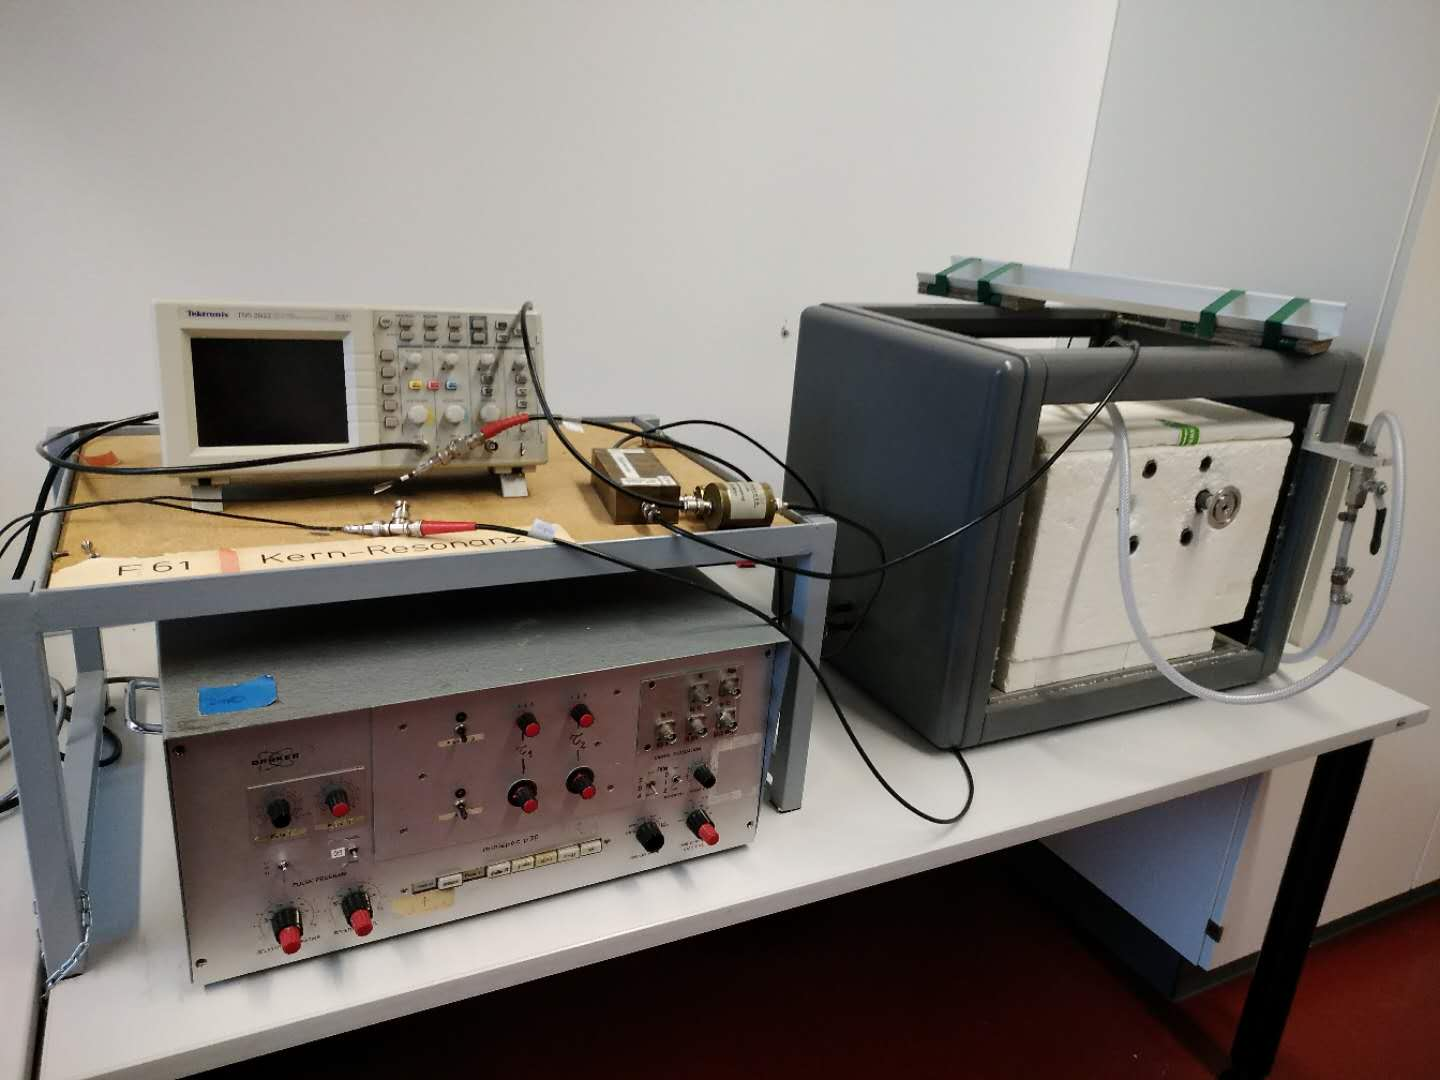
\includegraphics[scale=0.18]{images/minispec_p20.jpg}
	\caption{The minispec p20, electronic unit on the left, magnetic unit on the right}
	\label{mini}
\end{figure} \\
The constant $\vec{B_0}$, which is proportional to $\omega_{L}$, can be adjusted by turning the screw sticking out of the Styrofoam as seen in Figure \ref{mini} . The $\omega_{HF}$ will be set by the electronic unit of the p20 seen on the left side of Figure \ref{mini}. An oscilloscope is also provided to measure the characteristic time for a $90\degree$ pulse, which is needed to calibrate the electronic unit of the p20 for the relaxation time measurements. The tubes get inserted into the magnetic unit, parallel to the screw. A high-pressure air nozzle can be used to rotate the tube to ensure an evenly distributed density of the substance in the tube. \\
\begin{figure}[h!]
	\begin{subfigure}{0.32\textwidth}
	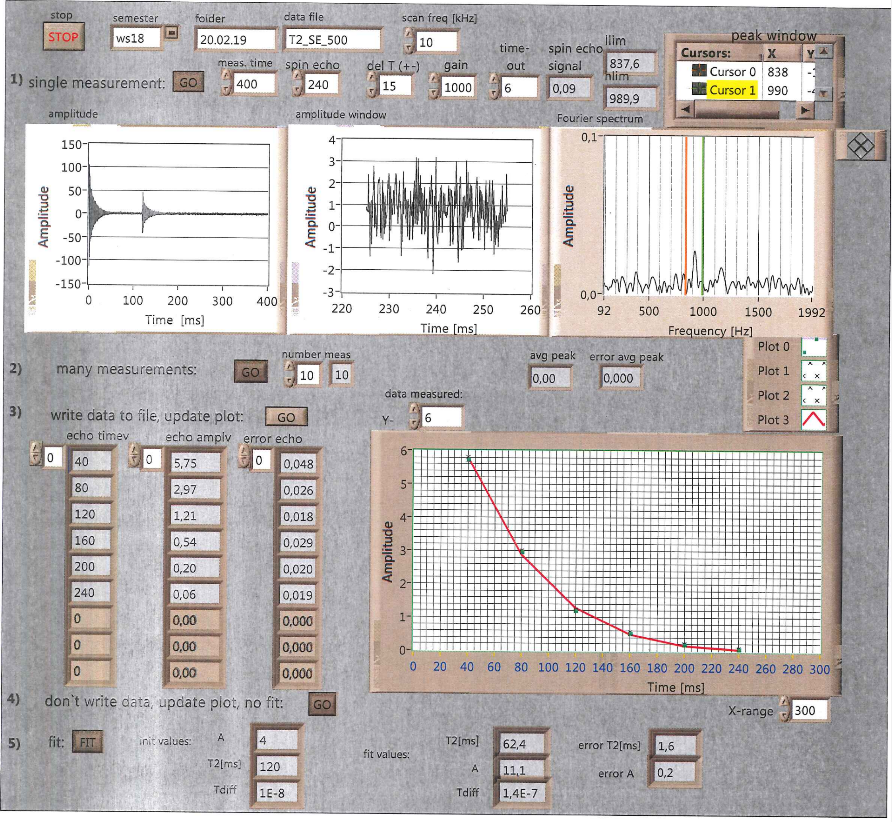
\includegraphics[width=0.9\linewidth ,height=4cm]{images/LabView1.png}
	\caption{Ga500 $T_2$ Spin-Echo}
	\label{Lab1}
	\end{subfigure}
	\begin{subfigure}{0.32\textwidth}
	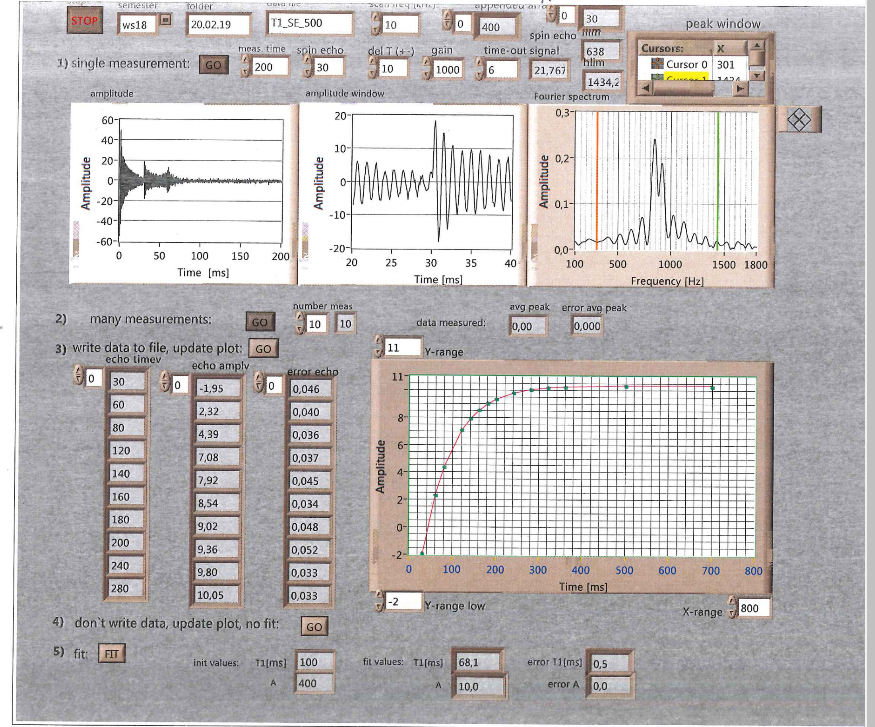
\includegraphics[width=0.9\linewidth ,height=4cm]{images/LabView3.png}
	\caption{Ga500 $T_1$ Spin-Echo}
	\label{Lab3}
	\end{subfigure}
	\begin{subfigure}{0.32\textwidth}
	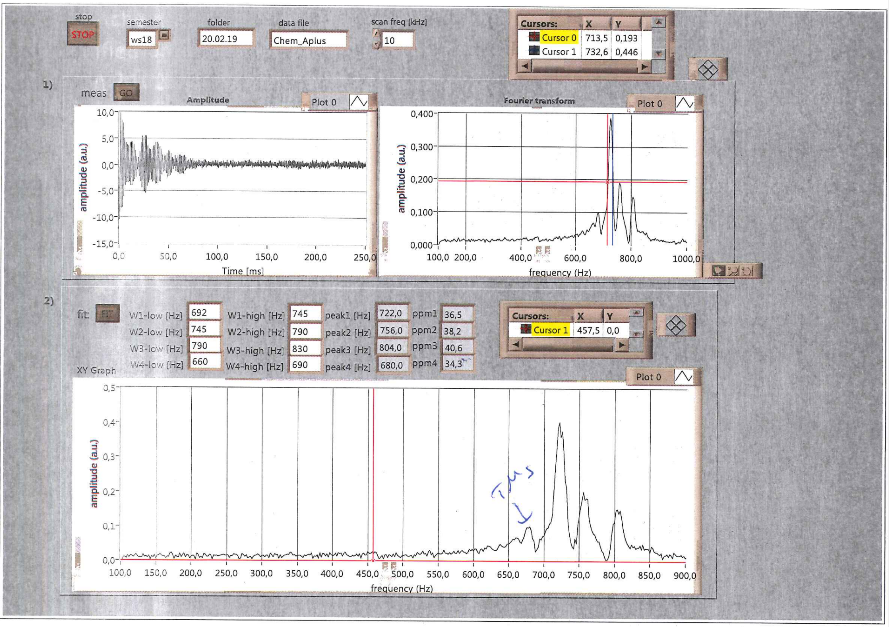
\includegraphics[width=0.9\linewidth, height=4cm]{images/LabView2.png}
	\caption{Chemical Shift}
	\label{Lab2}
	\end{subfigure}
	\caption{Example of the used Labviews}
	\label{exa}
\end{figure}\\
The data gets readout and analysed on a program written in Labview, the interface is shown in figure \ref{exa} via some example measurements.

\subsection{Imaging with NMR}\label{lay2}
We use a Bruker NMR analyzer 7.5 to generate the magnetic fields needed for 1D and 2D imaging. The readout gets fed into a computer where it gets analysed and can be later on displayed with a LabView .vi, examples of both can be seen in figure \ref{ImgLay}.
\begin{figure}[h!]
	\begin{subfigure}{0.5\textwidth}
	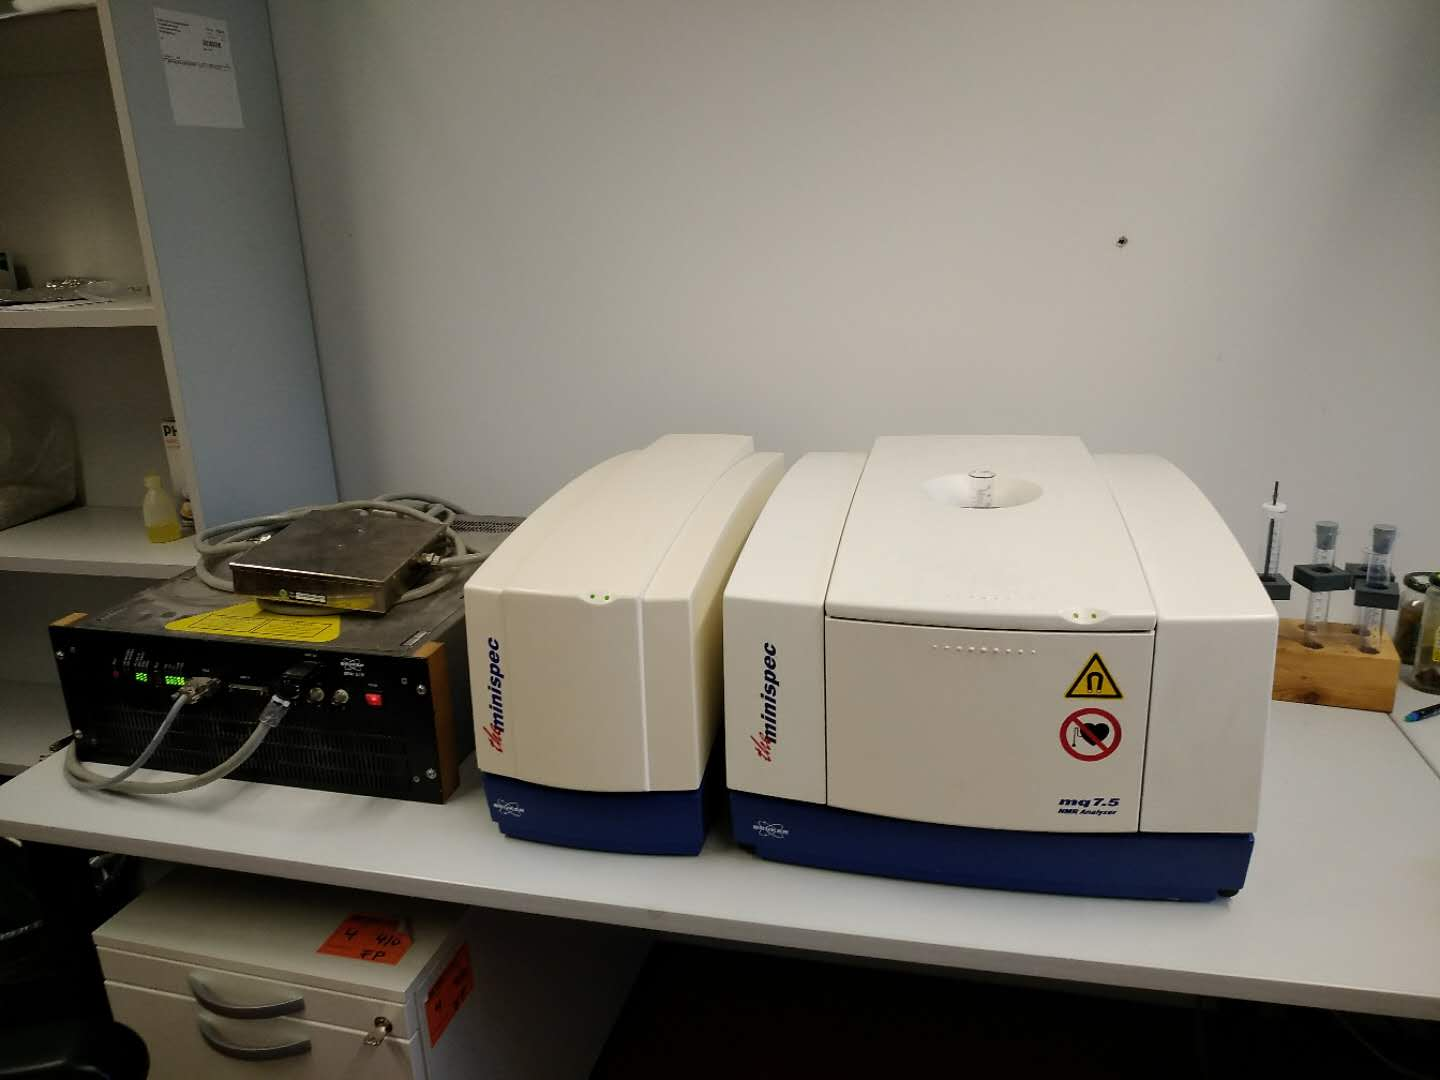
\includegraphics[width=0.9\linewidth ,height=4cm]{images/minispec_mq7_5.jpg}
	\caption{the Bruker NMR analyzer mq7.5}
	\label{Img1}
	\end{subfigure}
	\begin{subfigure}{0.5\textwidth}
	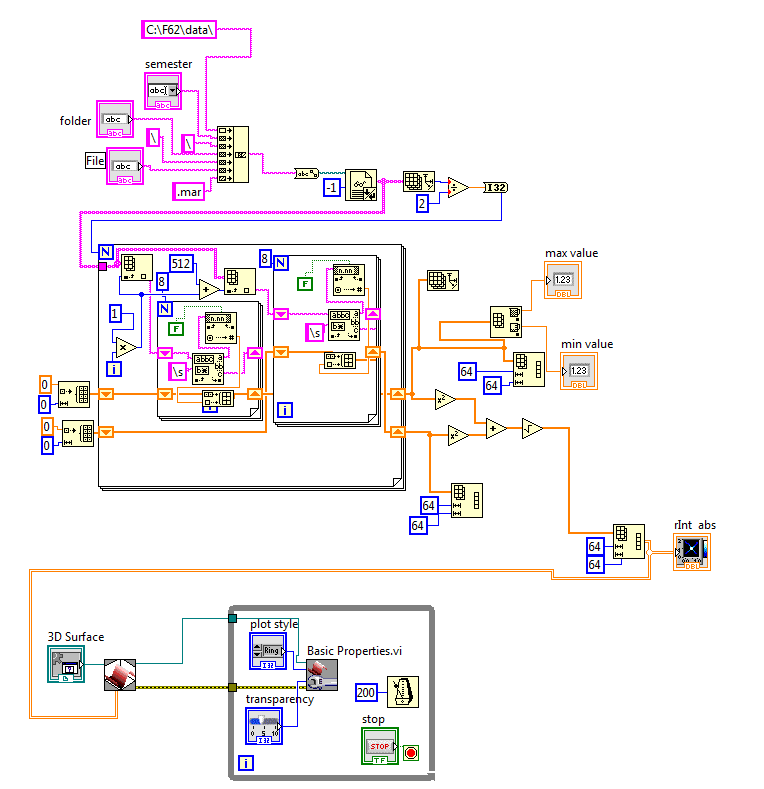
\includegraphics[width=0.5\linewidth ,height=4cm]{images/displaying_2d_image_labview_block.png}
	\caption{LabView .vi to display 2d image}
	\label{Img2}
	\end{subfigure}
	\caption{The NMR analyzer and LabView for 2D imaging}
	\label{ImgLay}
\end{figure}\\